% chktex-file 8
% chktex-file 13

\documentclass{article}
\usepackage{amsmath}
\usepackage{hyperref}
\usepackage{xcolor}
\usepackage{ulem}
\usepackage{graphicx}
\usepackage[margin=0.75in]{geometry}

\graphicspath{ {./images/} }

\definecolor{darkblue}{rgb}{0, 0, 20}

\hypersetup{
    colorlinks=true,
    urlcolor=darkblue,
    linkcolor=blue,
    filecolor=magenta,
    citecolor=blue,
}

\title{CoVR-2: Automatic Data Construction for Composed Video Retrieval}
\author{Lucas Ventura, Antoine Yang, Cordelia Schmid, Gul Varol}
\date{}
\setlength{\parindent}{0pt}

\begin{document}

\maketitle

\begin{center}\textbf{Accepted for TPAMI 2024 (\href{https://arxiv.org/pdf/2308.14746}{Paper}) (\href{https://github.com/lucas-ventura/CoVR/}{GitHub})}\end{center}

Composed image retrieval (CoIR) involves taking a source image and a modification prompt, and then retrieving a target image that reflects the modification to the image. Composed video retrieval (CoVR) applies the same thing, but retrieves a target video. This paper introduces a way to generate captions from videos in large datasets and then pairs the videos based on the similarity in the captions. They apply this method to the WebVid2M dataset to create the WebVid-CoVR dataset with 1.6 million triples. Lastly, they  demonstrate the transferability from CoVR to CoIR, achieving state-of-the-art zero-shot performance on the CIRR, FashionIQ, and CIRCO datasets after training on their WebVid-CoVR dataset.

\begin{center}
    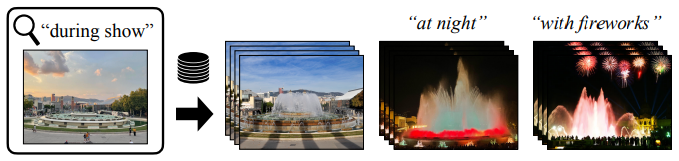
\includegraphics[scale=0.7]{covr2-1.png}
\end{center}

\section*{Motivation}

This method automatically pairs and annotates videos from a database, while previous methods required manual annotation and is unscalable. Also, there is a lack of large-scale CoVR datasets.

\section*{Method}

\subsection*{Automatic Triplet Generation}
\begin{enumerate}
    \item Videos from a video-caption dataset are paired based on the caption similarity, where captions are considered similar if there is only a one word difference.
    \item The caption pairs are filtered based on the CLIP text embedding similarity, only keeping the pair if similarity is between 0.6 and 0.96 to remove pairs that are too similar or too dissimilar.
    \item An LLM is fine-tuned on manually annotated triplets to generate modification texts from the source to target caption for the paired videos, which describes differences between the caption pairs.
\end{enumerate}

\begin{center}
    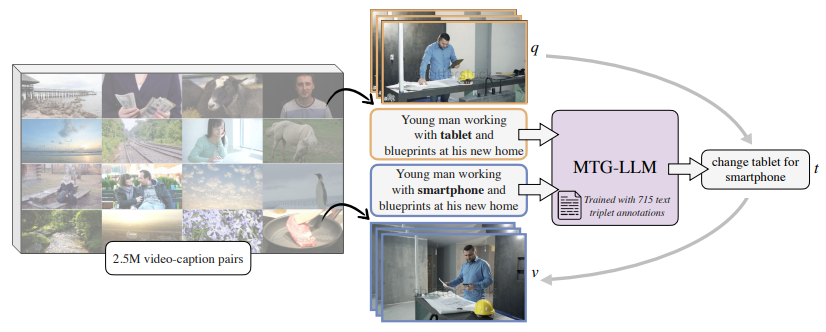
\includegraphics[scale=0.5]{covr2-2.png}
\end{center}

\subsection*{Dataset Generation}
\begin{enumerate}
    \item WebVid-CoVR is a CoVR training dataset with 1.6 million triplets generated with the previous method.
    \item WebVid-CoVR-Test is a small test dataset that is manually annotated. 3.2k video pairs are sampled from the WebVid10M dataset that aren't included in the WebVid2M dataset. For each of the pairs, the annotator manually creates one modification text and uses the LLM to generate two other modification texts for the same pair. The annotator then kept the best out of the three modification texts.
\end{enumerate}

\subsection*{CoVR-BLIP-2 Model}
\begin{enumerate}
    \item BLIP-2 is pretrained on a large dataset of image-caption pairs.
    \item The image encoder extracts visual features and the Q-Former module fuses visual and textual information to generate multi-modal query embeddings.
    \item A set of frames from a video are passed independently through the image encoder and then a weighted mean is applied to form the video embedding, where weights are computed based on text-image cosine similarity.
    \item At inference, the multi-modal query embedding for the source image and modification text and the video embeddings for all videos are computed. The video with the highest cosine similarity is retrieved.
    \item Uses Hard Negative Noise-Contrastive Estimation (HN-NCE) and Caption Retrieval to ensure the query embedding aligns with the correct target video and video caption, respectively.
\end{enumerate}

\begin{center}
    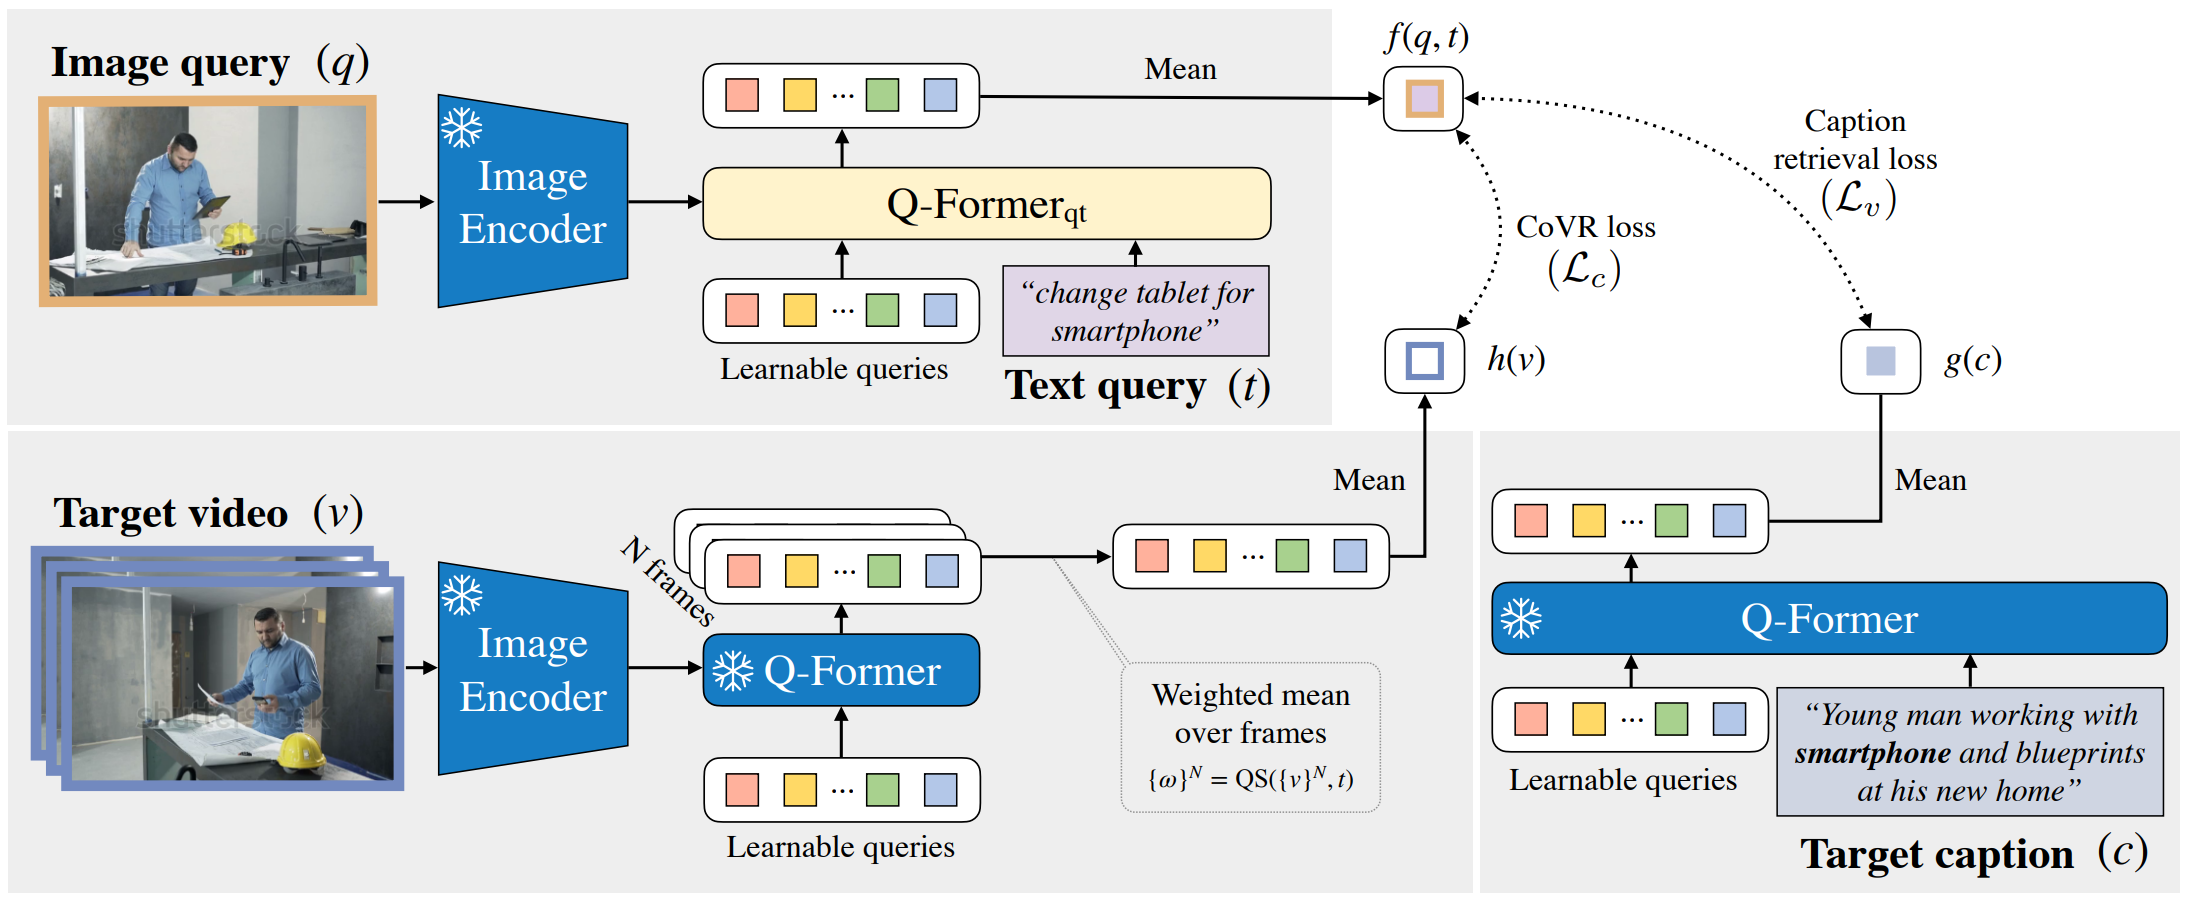
\includegraphics[scale=0.2]{covr2-3.png}
\end{center}

\section*{Limitations}
\begin{enumerate}
    \item The generated modification text does not consider visible changes in the images and only compares the captions.
    \item Captions are only considered similar if there is only a one word change but there may be similar captions with multi-word differences.
    \item 22\% of the samples in the test set were considered noisy and had to be discarded.
\end{enumerate}

\end{document}